\documentclass{article}
\usepackage[a4paper,]{geometry}
\usepackage{lmodern}
%\usepackage[export]{adjustbox}
\usepackage[utf8]{inputenc}
\usepackage[T1]{fontenc}
\usepackage{graphicx}
%\usepackage{titlepic}
\usepackage{mathtools}
%\usepackage{amsmath}
%\usepackage{amssymb}
%\usepackage{amsfonts}
%\usepackage{accents}
%\usepackage{esvect}
%\usepackage{subcaption}
\usepackage{multicol}
\usepackage{hyperref}
%\usepackage{enumitem}
\usepackage[makeroom]{cancel}
\usepackage{siunitx}
\usepackage{float}
\usepackage{lipsum}
\usepackage{textcomp}
\usepackage{circuitikz}
\usepackage{placeins}

\sisetup{separate-uncertainty=true}
\linespread{1.3}

% my commands
\newcommand{\E}[1]{\, \mathrm{e}{#1} \, }
\newcommand{\de}{\mathrm{d}}
\newcommand{\pars}{\mathbin{\!/\mkern-5mu/\!}}
\newcommand{\equalexpl}[1]{
	\underset{\substack{\uparrow\\\mathrlap{\text{#1}}}}{=}}


\title{Circuiti RLC}
\author{Filippo Dal Farra \and Matteo Zandegiacomo Orsolina}
\date{19 Novembre 2018}

\begin{document}

\maketitle

\newpage

\section{Introduzione}

Questa relazione riassume gli esiti di tre esperienze tutte finalizzate all'adempimento dell'analisi di un circuito RLC svolto durante l'ultima seduta. Per fare ci\'o si \'e sfruttato l'uso di un oscilloscopio il quale, da come si vedr\'a, modifica inevitabilmente le risposte dei circuiti in analisi. A causa di questo è risultato poi necessario derivare i valori delle capacità e delle resistenze parassite che si trovano all'interno dell'oscilloscopio per poi effettuare l'analisi tenendo conto di esse. \\

Successivamente abbiamo studiato la risposta in frequenza del circuito RC nelle diverse configurazioni di filtro passa alto e filtro passa basso, sempre variando le frequenze di taglio. Così facendo si \'e riusciti ad ottenere i diagrammi di Bode corrispondenti che associati alle relative funzioni di trasferimento teoriche forniscono i valori dei componenti usati nei vari casi. Inoltre queste misure sono poi state messe a confronto con i risultati ottenuti precedentemente nella carica e scarica del condensatore, per osservare se risultavano tra loro compatibili. \\

Infine abbiamo considerato anche un induttore, consistente in una bobina realizzata precedentemente. Inizialmente abbiamo studiato un circuito RL per trovate il valore dell'induttanza di questo elemento attraverso diversi cicli di carica e scarica del campo magnetico da esso generato. In seguito è stata posta all'interno di un circuito RLC composto dalla bobina e dal condensatore usato precedentemente di cui si sapeva a questo punto il valore. Ciò ci ha permesso di studiare il funzionamento del circuito passa banda e trovare la sua frequenza di risonanza. \\

Il codice utilizzato in questa esperienza \'e raggiungibile al \href{https://gitlab.com/volpx/lab-2/tree/master/Exp234}{<link>}.

\newpage

\section{Materiali e strumenti}

\begin{itemize}
  \item Varie resistenze da usare a seconda delle necessità
  \item Un condensatore
  \item Cavi "banana-banana"
  \item Breadboard
  \item Bobina precedentemente realizzata
  \item Multimetro digitale (DMM)
  \item Generatore di tensione variabile
  \item Oscilloscopio
  %\item %TODO: Non mi viene in mente altro, ma di sicuro ho dimenticato qualcosa
\end{itemize}

\newpage

\section{Procedure di misura}

Innanzitutto è stato necessario montare il circuito RC per osservare la scarica del condensatore come suggerito dalla scheda fornita \ref{fig:RC_LP}. Ad esso andava poi collegato l'oscilloscopio tramite i cavi coassiali all'ingresso ed all'uscita del circuito. Abbiamo impostato il generatore di funzioni in modo che  producesse lo scalino da $\Delta V$ a $0\ V$ , e in questa configurazione \'e stato osservato l'andamento in uscita dell'onda nella fase di scarica. Sono stati utilizzati 5 diversi valori di resistenza con lo stesso condensatore in modo da avere tempi caratteristici $\tau$ differenti e per ognuno sono state salvate 6 forme d'onda con l'oscilloscopio impostato a 16 averagings. Ciò ha fornito un numero sufficiente di dati per poi poter trovare i parametri relativi ad eventuali componenti parassiti, dato che in seguito la procedura \'e stata ripetuta senza il condensatore in esame, supplito dalla capacit\'a intrinseca di cavi e ADC dell'oscilloscopio. Tutti i valori di resistenza utilizzati sono stati misurati con il DMM. \\

Successivamente lo stesso circuito \'e stato studiato come filtro, analizzando la sua risposta ad un ingresso sinusoidale in funzione della frequenza applicata. Sono stati scelti valori di resistenza che ci dessero valori della frequenza di taglio specifici. Il generatore di funzioni \'e stato impostato a $V_{PP} = 2\div 4 V$ con frequenze distribuite esponenzialmente per una decade e \textonehalf \ prima e dopo la frequenza di taglio. Quindi sono stati da noi trascritti i valori di ampiezza in entrata ed uscita dal circuito assieme allo sfasamento tra i due forniti dall'oscilloscopio tramite le sue funzioni di misura in modo da poter creare il diagramma di Bode. Infine abbiamo applicato una resistenza in modo da caricare il circuito ed in queste condizioni \'e stata misurata l'impedenza in uscita del filtro con due diverse frequenze. La procedura è stato ripetuta con la configurazione passa alto \ref{fig:RC_HP1}, per un unico valore di resistenza. \\


In seguito si è considerata una bobina costruita precedentemente e con essa è stato costruito un circuito RL. Per fare ciò la bobina è stata inserita all'interno di un core di materiale ferromagnetico, il quale aveva il ruolo di amplificare l'induttanza da esso prodotta. Si è innanzitutto ancora usata un'onda quadra dal generatore di funzioni, con diverse configurazioni di resistenze in modo da studiarne la scarica. Si è poi montato un circuito RLC passa banda, sfruttando come induttore ancora la bobina e come condensatore l'elemento di circuito usato precedentemente. Si è impostato il generatore di funzioni in modo da realizzare un'onda sinusoidale applicata a due diverse configurazioni di valori di resistenza. Si è studiato ciò modificando i valori della frequenza, infittendo la risoluzione in concomitanza della frequenza di risonanza del circuito. \\

\newpage

%%%%%%%%%%%%% ANAL-isis %%%%%%%%%%%%%%%%%%%

\section{Analisi dei dati}

Verranno ora analizzati i dati ottenuti per ogni configurazione.

\subsection{Scarica condensatore}

Il circuito ora preso in considerazione \'e il seguente:

\begin{figure}[h]
\begin{center}
    \begin{circuitikz} []
    \draw
        node[ground] (0,0) {} to [sqV] (0,2) to [R, l=$R_s$] (2,2)
        (4,0) node[ground] {} to [C, l=$C$] (4,2)
        (6,0) node[ground] {} to [C, l=$C_{osc}$] (6,2)
        (8,0) node[ground] {} to [R, l=$R_{osc}$] (8,2)
        (2,2) to [R, l=$R$] (4,2) to (9,2)  node[right]{$V_{out}$} 
        (2,2) to (2,3) to (9,3) node[right]{$V_{in}$}
        (9,2) to [open, *-*] (9,3);
    \end{circuitikz}
    \caption{Circuito RC passa basso utilizzato anche per l'analisi della scarica del condensatore}
    \label{fig:RC_LP}
\end{center}
\end{figure}


Utilizzando la legge di Kirchhoff per le tensioni e presa la maglia passante per resistenza $R$ e condensatore $C$ e considerando la relazione tra corrente e tensione ai capi di esso \ref{eq:cap_law} si ottiene l'equazione differenziale \ref{eq:cap_equ} che rappresenta una semplificazione di quello che accade nel nostro circuito nell'approssimazione $C_{osc}=0$ e $R_{osc} = \infty $.

\begin{gather}
    i(t) = C \frac{\de V_c (t)}{\de t}
    \label{eq:cap_law} \\   
    \nonumber V_{in} - i(t) R - V_c(t) = 0 \Rightarrow \\
    \tau \frac{\de V_c(t)}{\de t} + V_c(t) = V_{in} \quad \textrm{con} \quad \tau = RC
    \label{eq:cap_equ}
\end{gather}

Date le condizioni iniziali di condensatore carico a $V_c(t = 0) = \Delta V$ che \'e il livello di tensione alta del generatore di funzioni il quale per $t > 0$ fornisce $V_{in} = 0$ si ottiene la forma analitica della scarica del condensatore \ref{eq:cap_dis} risolvendo l'equazione differenziale corrispondente.

\begin{gather}
	\nonumber 
	\frac{\de V_c(t)}{\de t} = - \frac{1}{\tau} V_c(t) \\
	V_c(t) = \Delta V \exp{- \frac{t}{\tau}}
	\label{eq:cap_dis}
\end{gather}

Tuttavia l'applicazione del circuito di misura, l'oscilloscopio nel nostro caso, e la presenza della resistenza in uscita del generatore provocano inevitabilmente una modifica del caso ideale, in particolare $R_{osc}$ fa un partitore di tensione con $R$ e $R_{s}$ cos\'i che il condensatore non \'e inizialmente carico alla tensione del generatore e la sua scarica avviene anche attraverso $R_{osc}$.
L'equazione \ref{eq:cap_dis} si sostituisce quindi con l'equazione \ref{eq:cap_dis_real} che tiene conto dei componenti parassiti.

\begin{gather}
	\nonumber 
	V_0 = \Delta V \frac{R_{osc}}{R_{osc} + R + R_{s}} \\ 
	\tau = ( C_{osc} + C ) ( (R + R_s) \pars R_{osc} ) \\
	V_{out}(t) = V_c(t) = V_0 \exp{ -\frac{t}{\tau} }
	\label{eq:cap_dis_real}
\end{gather}

A scopo rappresentativo viene quindi mostrata una delle forme campionate:

\begin{figure}[h]
    \centering
    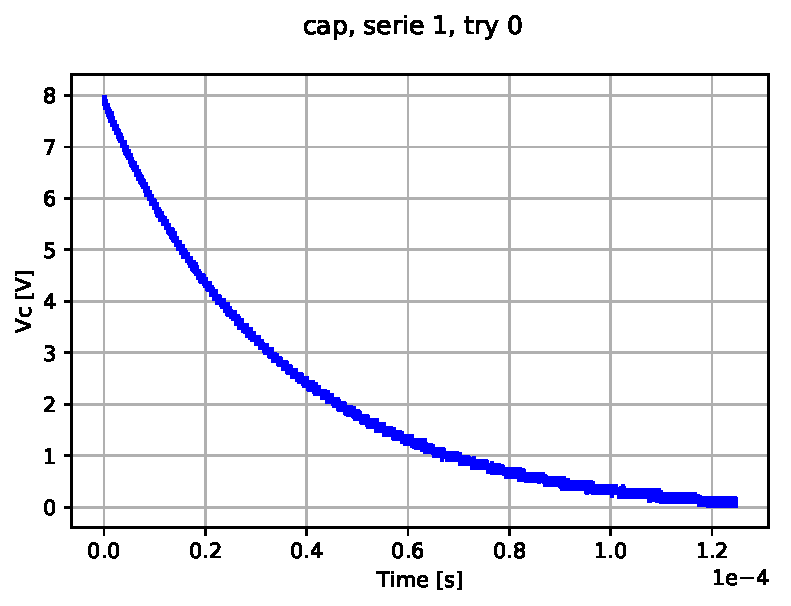
\includegraphics[width = 0.5\textwidth]{capserie1try0.pdf}
    \caption{Primo campione preso con il primo valore di resistenza, si nota qualitativamente che la scarica \'e compatibile con una caduta esponenziale}
    \label{fig:cap_dis_ex}
\end{figure}

La relazione \ref{eq:cap_dis_real} che rappresenta la scarica del condensatore in funzione del tempo pu\'o essere linearizzata in questa variabile se viene preso il logaritmo di $V_{out}$ \ref{eq:cap_dis_lin}.

\begin{gather}
	\ln{V_{out}(t)} = \ln{ \left( V_0 \exp{ -\frac{t}{\tau} } \right) } = \ln{V_0} + \left( -\frac{1}{\tau} \right) t = A + B t \\
	\sigma[\ln{V_{out}}]=\frac{\sigma[V_{out}]}{V_{out}}
	\label{eq:cap_dis_lin}
\end{gather}

\begin{figure}[h]
    \centering
    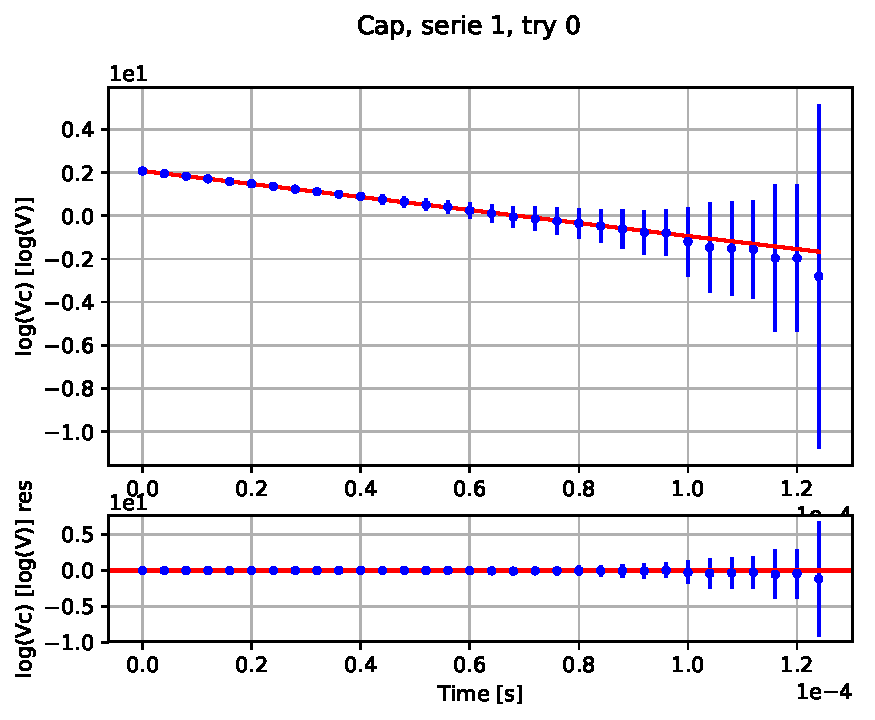
\includegraphics[width = 0.5\textwidth]{fitplot6.pdf}
    \caption{Esempio di fit della scarica del condensatore, in blu i dati misurati, un punto ogni 400 per questioni di chiarezza, ed in rosso il risultato della regressione lineare.}
    \label{fig:cap_dis_ex_lin}
\end{figure}

Si pu\'o quindi procedere al fit lineare per il calcolo dei parametri $A$ e $B$ e il risultato con il confronto tra modello e campioni \'e mostrato in figura \ref{fig:cap_dis_ex_lin}. Come si pu\'o vedere, avvicinandosi a $V_c = 0$ i campioni presi mostrano un drift dal modello: questo \'e molto probabilmente dovuto ad un offset sullo zero dell'oscilloscopio e tale ipotesi viene quindi ora analizzata.

La presenza di un offset $\delta V$, assunto fisso, in fase di misura non ci permette di applicare la regressione lineare del caso precedente: 

\begin{gather}
	\nonumber
	V_m(t) = V_{out}(t) + \delta V =  V_0 \exp{ -\frac{t}{\tau} } + \delta V
	\\
	\nonumber
	\ln{V_m(t)} \equalexpl{\hspace{-2.5em}$V_{out} \approx V_m$} 
	\ln{\left( V_0 \exp{ -\frac{t}{\tau} } \right) } + 
	\ln{\left( 1 + \frac {\delta V}{V_{m}} \right) } = 
	\\
	\nonumber
	\equalexpl{\hspace{-4.5em}$\ln(1+x) = x + o(x)$} 
	\ln{\left( V_0 \exp{ -\frac{t}{\tau} } \right) } + 
	\frac {\delta V}{V_m} = A + B t + C\frac{1}{V_m}
	\\
	A = \ln{V_0} \quad B = -\frac{1}{\tau} \quad C = \delta V
	\label{eq:gen_reg}
\end{gather}  

Si procede quindi ad applicare la regressione generalizzata \ref{eq:gen_reg}. Dato che per ogni valore di resistenza sono state registrate 6 scariche del condensatore si estraggono poi i tre  parametri come funzione della sola resistenza applicata effettuando la media campionaria sui 6 valori ottenuti ed i risultati sono esposti in tabella \ref{tab:ABC1}.



\begin{figure}[h]
\begin{center}
	\large{Con condensatore}
	
	\begin{tabular}{c|c c c} 
	$R$ [\si{\ohm}] & $A$ [log(\si{\volt})] & $B$ [\si{\per\second}] & $C$ [\si{\volt}] \\
	[0.5ex]
	\hline
	$ 998.2 $&$ 2.07683\pm 0.00011 $&$ -28986\pm 6 $&$ -0.09284\pm 0.00024 $\\
	$ 9917.0 $&$ 2.07150\pm 0.00009 $&$ -3068.8\pm 0.6 $&$ -0.09144\pm 0.00012 $\\
	$ 99660.0 $&$ 1.9875\pm 0.0005 $&$ -336.58\pm 0.20 $&$ -0.0640\pm 0.0006 $\\
	$ 29820.0 $&$ 2.04916\pm 0.00010 $&$ -1044.13\pm 0.24 $&$ -0.08552\pm 0.00019 $\\
	$ 373200.0 $&$ 1.7690\pm 0.0004 $&$ -114.31\pm 0.09 $&$ -0.0307\pm 0.0005 $\\
	
	\end{tabular}
	
	
	\vspace{0.5cm}
	
	\large{Senza condensatore}
		
	\begin{tabular}{c|c c c} 
	$R$ [\si{\ohm}] & $A$ [log(\si{\volt})] & $B$ [\si{\per\second}] & $C$ [\si{\volt}] \\
	[0.5ex]
	\hline
	$ 998.2 $&$ 2.1503\pm 0.0012 $&$ (-6.840\pm 0.012)\E{6} $&$ -0.1958\pm 0.0022 $\\
	$ 9917 $&$ 2.0561\pm 0.0009 $&$ (-7.5257\pm 0.0031)\E{5} $&$ -0.0733\pm 0.0007 $\\
	$ 99660 $&$ 1.95850\pm 0.00021 $&$ -80567\pm 18 $&$ -0.08907\pm 0.00016 $\\
	$ 29820 $&$ 2.0384\pm 0.0006 $&$ (-2.5736\pm 0.0007)\E{5} $&$ -0.0877\pm 0.0005 $\\
	$ 373200 $&$ 1.73688\pm 0.00023 $&$ -27803\pm 28 $&$ -0.03462\pm 0.00016 $\\
	
	\end{tabular}
\end{center}
\label{tab:ABC1}
\end{figure}

Per estrarre il valore della capacit\'a in esame si procede all'analisi del parametro $B$ nei due casi che risulta avere la seguente relazione, in cui $R_s = 50\ \si{\ohm}$ \'e l'impedenza in uscita dal generatore di funzioni in serie con la resistenza $R$. \\

\begin{equation}
	-B=\frac{1}{\tau}=\frac{1}{C} \left( \frac{1}{R+R_s} + \frac{1}{R_{osc}} \right) = \gamma + \lambda \frac{1}{R+R_s}
\end{equation}
\\
Si effettua un plot \ref{fig:fit1} per mostrare la relazione tra $1/\tau$ in funzione della conduttanza $1/R_{tot}$ applicata nei casi con e senza condensatore incognito assieme alla corrispondente regressione lineare con i parametri $\gamma$ e $\lambda$.

\begin{figure}[h]
	\centering
	 \begin{minipage}{0.5\textwidth}
	     \centering
	     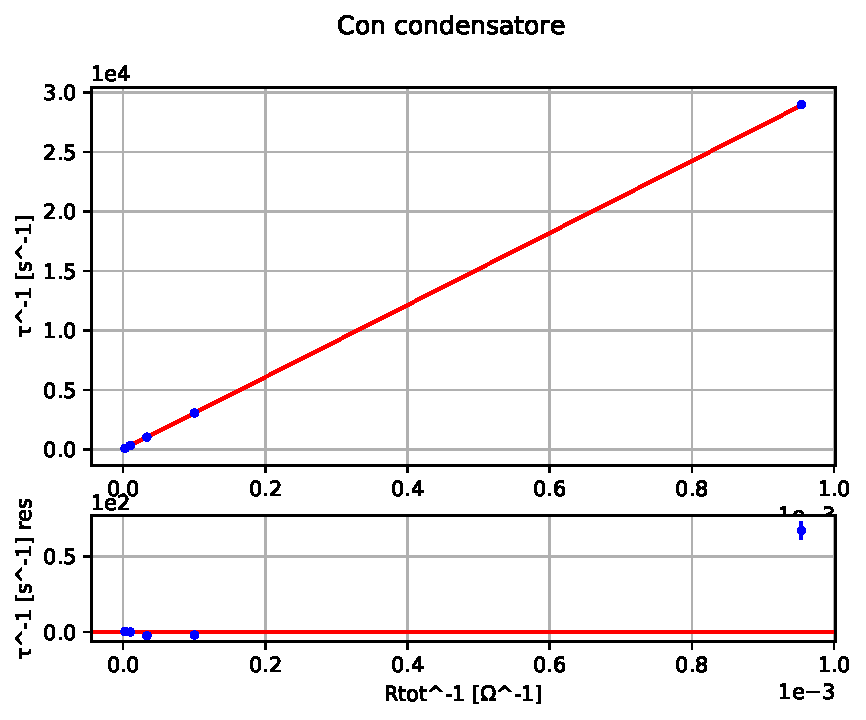
\includegraphics[width=\textwidth]{figfit.pdf}
	     %\caption{first figure}
	 \end{minipage}\hfill
	 \begin{minipage}{0.5\textwidth}
	     \centering
	     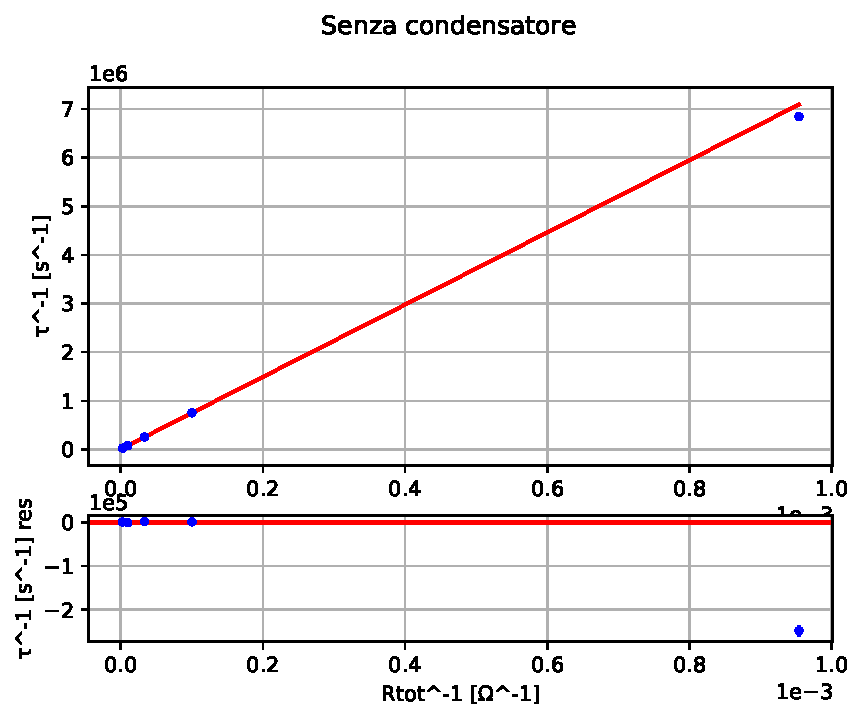
\includegraphics[width=\textwidth]{figfit1.pdf} 
	     %\caption{second figure}
	 \end{minipage}
	 \caption{plot che lega 1/$\tau$ a 1/R}
	 \label{fig:fit1}
\end{figure}

\begin{center}
\begin{tabular}{c | c c} 
& Con condensatore  & Senza condensatore \\
[0.5ex]
\hline
$C_{tot}=1/\lambda \ [\si{\farad}]$ &$ (3.3026\pm 0.0004)\E{-8} $&$ (1.34727\pm 0.00034)\E{-10} $\\
$R_{osc}=\lambda/\gamma \ [\si{\ohm}]$ &$ (9.22\pm 0.08)\E{5} $&$ (1.0946\pm 0.0008)\E{6} $\\
$\chi^2_{r,\mathrm{3 dof}}$& $85.15$ & $13.78\E{6}$ \\

\end{tabular}
\end{center}

Come \'e evidente, il valore del $\chi^2$ ottenuto mostra un'incompatibilit\'a con tra le misure ottenute e il modello teorico. Questo potrebbe essere spiegato dal fatto che ci siano degli effetti che non sono stati presi in considerazione. Scegliamo quindi di considerare veritiera la legge teorica e conseguentemente scalare le incertezze, le quali erano quindi state sottostimate, in modo da imporre $\chi^2_r=1$.\\

\begin{center}
\begin{tabular}{c | c c} 
& Con condensatore  & Senza condensatore \\
[0.5ex]
\hline
$C_{tot}=1/\lambda \ [\si{\farad}]$ &$ (3.303\pm 0.004)\E{8} $&$ (1.3\pm 1.3)\E{-10} $\\
$R_{osc}=\lambda/\gamma \ [\si{\ohm}]$ &$ (9.22\pm 0.25)\E{5} $&$ (1.09\pm 0.05)\E{6} $\\
\end{tabular}
\end{center}

Otteniamo quindi i parametri del circuito in esame, considerando nel caso delle due $R_{osc}$ la media dei due valori con incertezza corrispondente alla loro deviazione standard: \\

\begin{gather}
	\nonumber
	C=(3.289\pm 0.013)\E{8}\\
	\nonumber
	C_{osc}=(1.3\pm 1.3)\E{-10} \\
	\nonumber
	R_{osc}=(1.01\pm 0.08)\E{6} \\
\end{gather}

\newpage
%%%%%%%%%%%%%%%%%%%% FILTRI RC %%%%%%%%%%%%%%%%%%%%%%%%
\subsection{Filtri RC}

Si analizza ora la risposta in frequenza del circuito \ref{fig:RC_LP1} e del circuito \ref{fig:RC_HP1}.

\begin{figure}[h]
\begin{center}
    \begin{circuitikz} []
    \draw
        (0,0) node[ground] {} to [sV] (0,2) to [R, l=$R_s$] (2,2)
        (4,0) node[ground]  {}  to [C, l=$C$] (4,2)
        (6,0) node[ground]  {} to [C, l=$C_{osc}$] (6,2)
        (8,0) node[ground]  {} to [R, l=$R_{osc}$] (8,2)
        (2,2) to [R, l=$R$] (4,2) to (9,2) node[right]{$V_{out}$}
        (2,2) to (2,3) to (9,3) node[right]{$V_{in}$}
        (9,2) to [open, *-*] (9,3);
    \end{circuitikz}
\end{center}
\caption{Curcuito RC Low Pass}
\label{fig:RC_LP1}
\end{figure}

\begin{figure}[h]
\begin{center}
    \begin{circuitikz} []
    \draw
        (0,0) node[ground] {} to [sV] (0,2) to [R, l=$R_s$] (2,2)
        (4,0) node[ground] {} to [R, l=$R$] (4,2)
        (6,0) node[ground] {} to [C, l=$C_{osc}$] (6,2)
        (8,0) node[ground] {} to [R, l=$R_{osc}$] (8,2)
        (2,2) to [C, l=$C$] (4,2) to (9,2) node[right]{$V_{out}$}
        (2,2) to (2,3) to (9,3) node[right]{$V_{in}$}
        (9,2) to [open, *-*] (9,3);
    \end{circuitikz}
\end{center}
\caption{Curcuito RC High Pass}
\label{fig:RC_HP1}
\end{figure}

Le funzioni di trasferimento senza il contributo di $C_{osc}$ e $R_{osc}$, in prima analisi trascurabili, risultano essere:

\begin{gather}
	H(\omega) = \frac{V_{out}}{V_{in}} = \frac{1}{1+j \omega \tau} \quad \tau=RC \\
	H(\omega)  = \frac{j \omega \tau}{1+j \omega \tau} \quad \tau=RC
\end{gather}

Dove $C=(3.289\pm 0.013)\E{8}$ \'e il condensatore utilizzato nell'analisi precedente.

Vengono quindi graficati modulo e fase dei dati misurati a confronto con la risposta teorica per i tre valori di frequenza di taglio scelti:

\begin{figure}[H]
    \centering
    \begin{minipage}{0.5\textwidth}
        \centering
        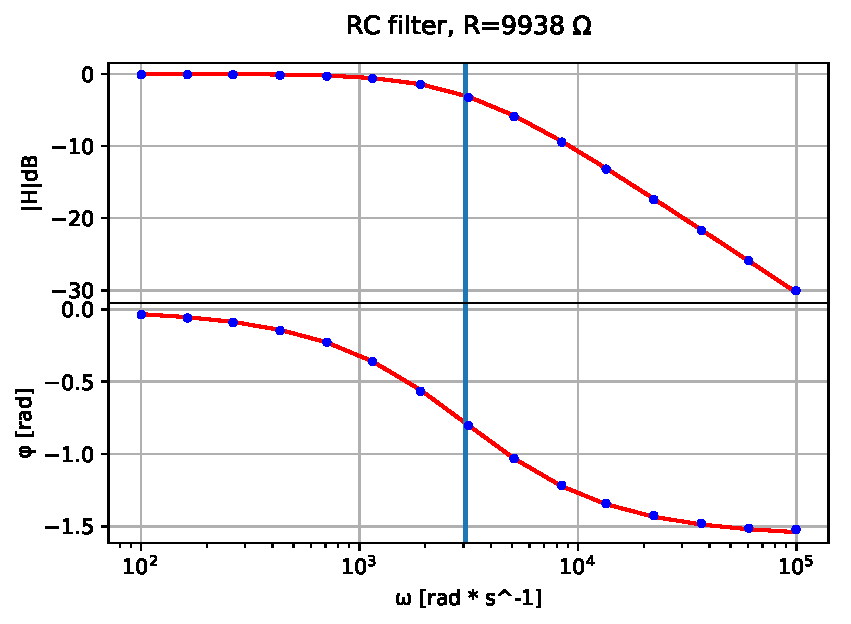
\includegraphics[width=\textwidth]{bodeplot1.pdf} 
        %\caption{first figure}
    \end{minipage}\hfill
    \begin{minipage}{0.5\textwidth}
        \centering
        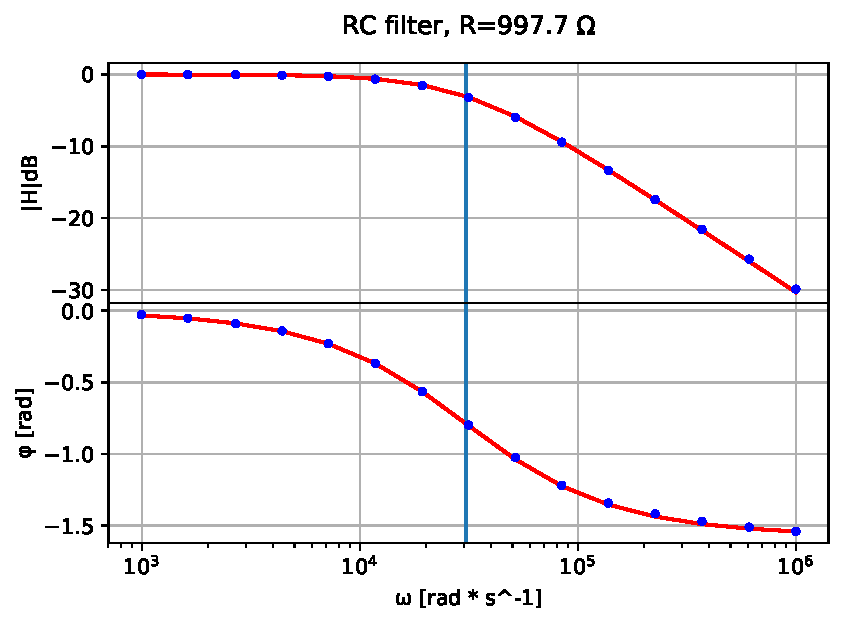
\includegraphics[width=\textwidth]{bodeplot2.pdf} 
        %\caption{second figure}
    \end{minipage}
    \\
    \centering
    \begin{minipage}{0.5\textwidth}
        \centering
        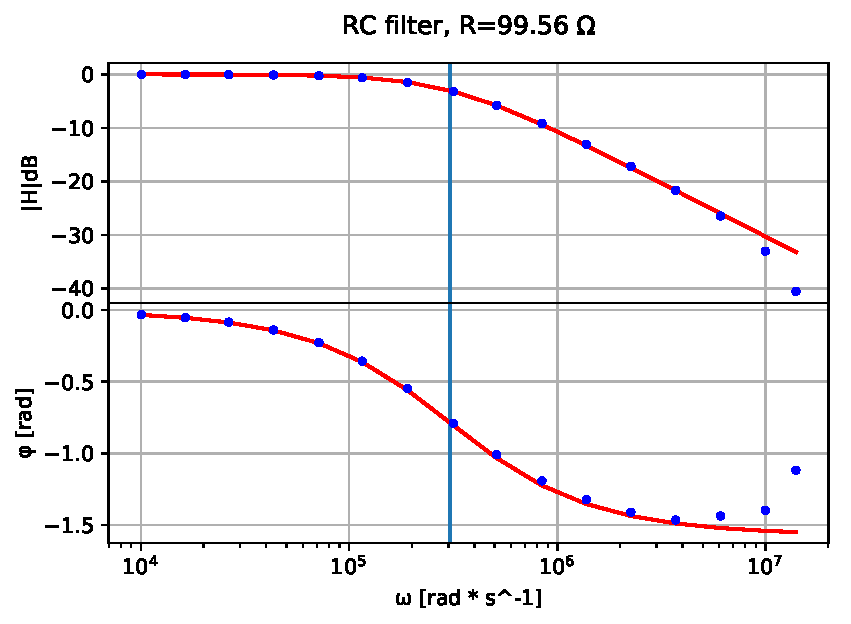
\includegraphics[width=\textwidth]{bodeplot3.pdf} 
        %\caption{first figure}
    \end{minipage}\hfill
    \begin{minipage}{0.5\textwidth}
        \centering
        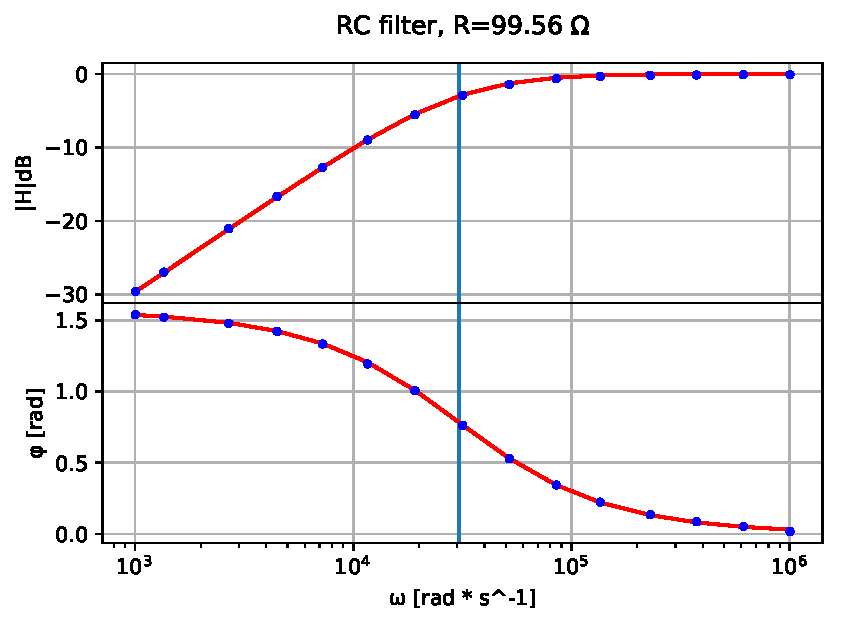
\includegraphics[width=\textwidth]{bodeplot4.pdf} 
        %\caption{second figure}
    \end{minipage}
    \caption{Grafici dei tre filtri Low Pass e del filtro High Pass accostati alle loro previsioni teoriche, la linea verticale azzurra mostra la posizione della frequenza di taglio teorica}
    \label{fig:RC_fil}
\end{figure}

\begin{figure}[H]
    \centering
    \begin{minipage}{0.5\textwidth}
        \centering
        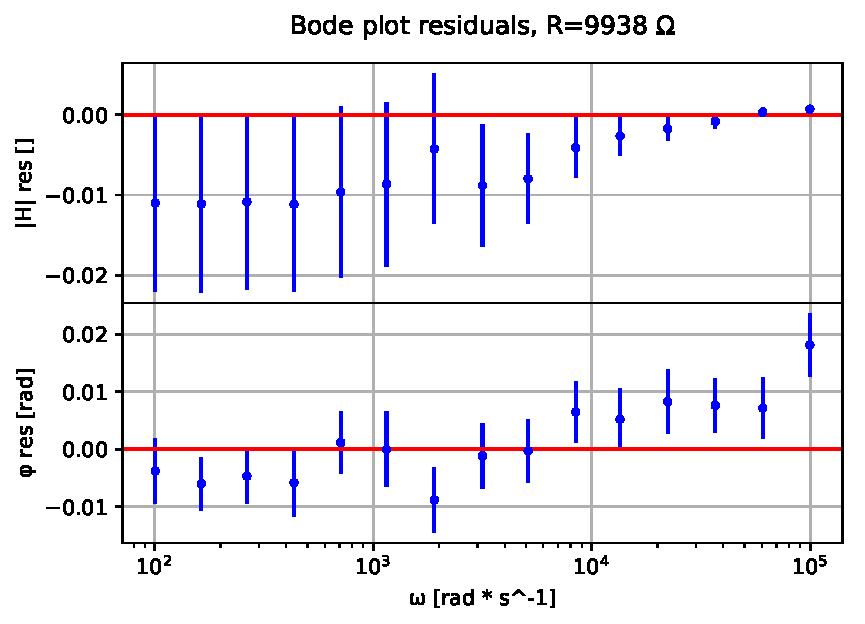
\includegraphics[width=\textwidth]{bodeplot_res1.pdf} 
        %\caption{first figure}
    \end{minipage}\hfill
    \begin{minipage}{0.5\textwidth}
        \centering
        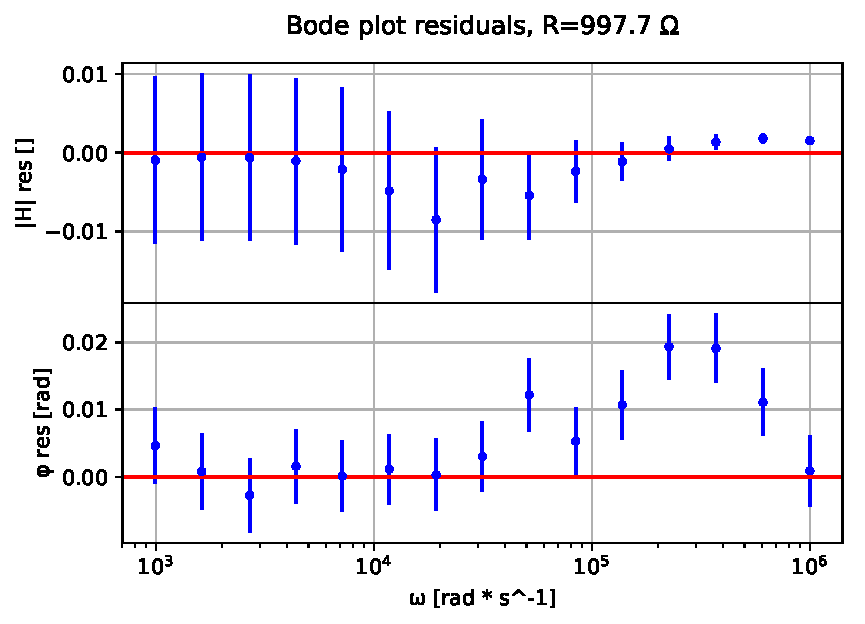
\includegraphics[width=\textwidth]{bodeplot_res2.pdf} 
        %\caption{second figure}
    \end{minipage}
    \\
    \centering
    \begin{minipage}{0.5\textwidth}
        \centering
        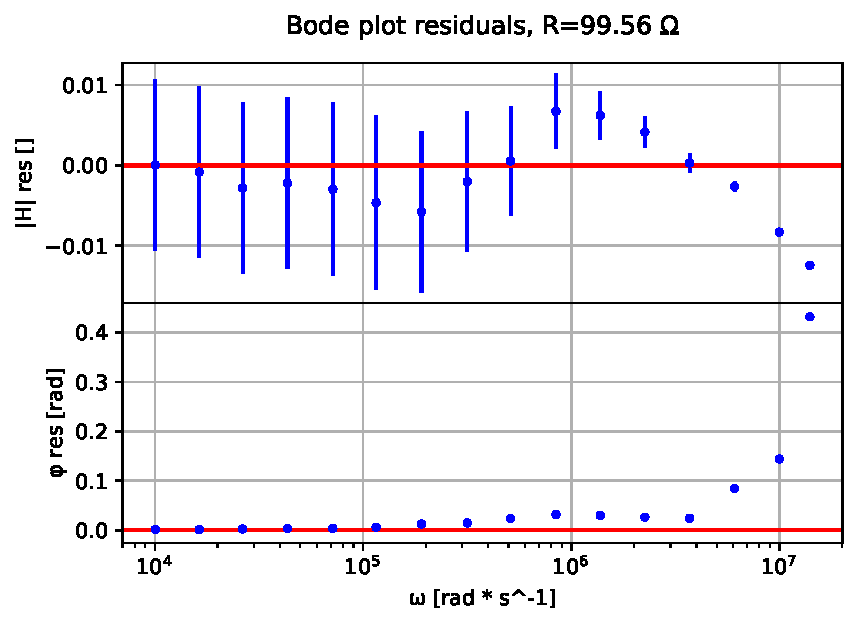
\includegraphics[width=\textwidth]{bodeplot_res3.pdf} 
        %\caption{first figure}
    \end{minipage}\hfill
    \begin{minipage}{0.5\textwidth}
        \centering
        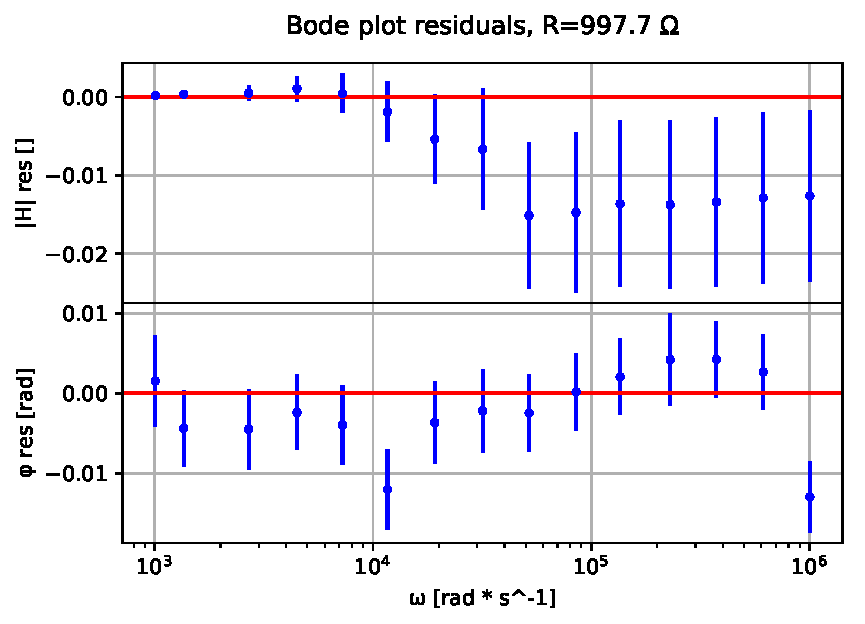
\includegraphics[width=\textwidth]{bodeplot_res4.pdf} 
        %\caption{second figure}
    \end{minipage}
    \caption{Residui dei grafici di Bode dei filtri passa basso e passa alto}
    \label{fig:RC_fil_res}
\end{figure}

Come si vede dai grafici \ref{fig:RC_fil} e \ref{fig:RC_fil_res} il modello teorico mostra una notevole compatibilit\'a con i dati raccolti a meno di effetti di ordine superiore che causano deviazioni comunque minime dovute probabilmente al non aver considerato le componenti parassite $R_{osc}$ e $C_{osc}$ per il calcolo della funzione di trasferimento. Un'eccezzione si vede sul grafico corrispondente a $R=99.56 \si{\ohm}$ il quale per frequenze maggiori di $\omega = 3\ \si{\mega\radian\per\second}$ mostra una deviazione molto pi\'u marcata ma comunque spiegabile dalla presenza di componenti parassiti nel circuito che agiscono solamente a frequenze cos\'i alte.

\FloatBarrier
\newpage

\subsection{Scarica Induttanza}

Si procede ora ad analizzare il comportamento dell'induttanza nel circuito \ref{fig:RL_circ} nella fase di scarica della stessa. Verranno inoltre trascurate le capacità parassite eventualmente presenti, nonch\'e la resistenza interna dell'oscilloscopio verso massa essendo in parallelo ad $R$ di valore molto pi\'u piccolo.

\begin{figure}[h]
%\renewcommand{\arraystretch}{9}
%\renewcommand{\arraystretch}{9}
\begin{center}
    \begin{circuitikz} []
    \draw
        (0,0) node[ground] {} to [sqV] (0,2) to [R, l=$R_s$] (2,2)
        (6,0) node[ground] {} to [R, l=$R$] (6,2)
        (4,2) to [R, l=$R_{l}$] (2,2)
        (4,2) to [L, l=$L$, i=i] (6,2) to (8,2) node[right]{$V_{out}$}
        (2,2) to (2,3) to (8,3) node[right]{$V_{in}$}
        (8,2) to [open, *-*] (8,3);
    \end{circuitikz}
\end{center}
\caption{Circuito RL}
\label{fig:RL_circ}
\end{figure}

Quando $V_{gen}=\Delta V$ \'e al livello alto ed il transiente \'e finito, $L$ mostra un'impedenza nulla e:

\begin{gather}
	V_{out}=V_{gen} \frac{R}{R  + R_l + R_s} \\
	i = \frac{ V_{gen} }{ R + R_l + R_s}
\end{gather}

Nel momento in cui il generatore passa al livello basso di potenziale $V_{gen}=0\si{\volt}$ si assiste ad una curva di scarica esponenziale della tensione $V_{out}$ e quindi della corrente $i$ che scorre in $R$.

\begin{gather}
	V_{out} = V_{0} \exp{-\frac{t}{\tau}}\\
	\nonumber
	V_0 = \Delta V \frac{R}{R_{s} + R_l + R}\\
	\nonumber
	\tau = \frac{L}{ R_{s} + R_l + R }
\end{gather}

\begin{figure}
\centering
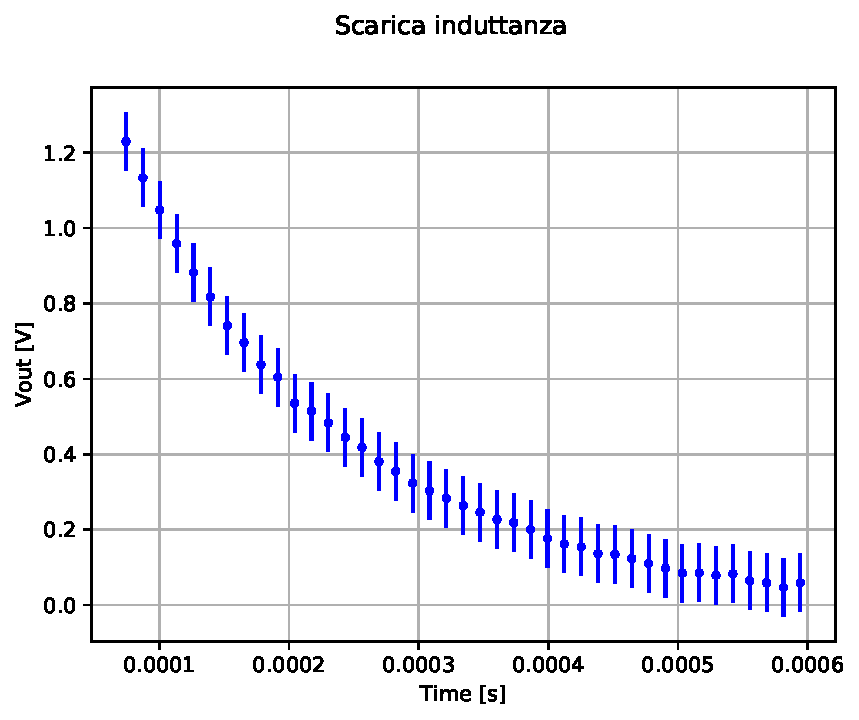
\includegraphics[width=0.5\textwidth]{ind_dis.pdf}
\label{fig:L_dis}
\caption{Curva di scarica esponenziale dell'induttore}
\end{figure}

Come \'e stato fatto nel caso della scarica del condensatore viene quindi eseguito il fit \ref{eq:gen_reg1} per la determinazione dei parametri considerando ancora una volta un offset sulla misura dell'oscilloscopio.

\begin{gather}
	\nonumber
	V_m(t) = V_{out}(t) + \delta V =  V_0 \exp{ -\frac{t}{\tau} } + \delta V
	\\
	\nonumber
	\ln{V_m(t)} \equalexpl{\hspace{-2.5em}$V_{out} \approx V_m$} 
	\ln{\left( V_0 \exp{ -\frac{t}{\tau} } \right) } + 
	\ln{\left( 1 + \frac {\delta V}{V_{m}} \right) } = 
	\\
	\nonumber
	\equalexpl{\hspace{-4.5em}$\ln(1+x) = x + o(x)$} 
	\ln{\left( V_0 \exp{ -\frac{t}{\tau} } \right) } + 
	\frac {\delta V}{V_m} = A + B t + C\frac{1}{V_m}
	\\
	A = \ln{V_0} \quad B = -\frac{1}{\tau} \quad C = \delta V
	\label{eq:gen_reg1}
\end{gather}

I risultati ottenuti per ogni ripetizione dell'acquisizione con la stessa resistenza vengono mediati e qui esposti: 

\begin{center}
\begin{tabular}{c|c c c} 
	$R$ [\si{\ohm}] & $A$ [log(\si{\volt})] & $B$ [\si{\per\second}] & $C$ [\si{\volt}] \\
	[0.5ex]
	\hline
	$ 20.16 $&$ 0.6361\pm 0.0010 $&$ -6022\pm 13 $&$ 0.0063\pm 0.0007 $ \\
	$ 46.17 $&$ 1.2051\pm 0.0005 $&$ -7994\pm 8 $&$ -0.0044\pm 0.0005 $ \\
	$ 98.8 $&$ 1.59056\pm 0.00023 $&$ -12099\pm 5 $&$ -0.0247\pm 0.0006 $ \\
	$ 149.4 $&$ 1.72880\pm 0.00011 $&$ -16136.2\pm 3.5 $&$ -0.0281\pm 0.0006 $ \\
	$ 198.3 $&$ 1.79624\pm 0.00018 $&$ -19984\pm 6 $&$ -0.0298\pm 0.0005 $ \\
\end{tabular}
\end{center}

Concentrandoci ora su B, si procede quindi ad effettuare un grafico \ref{fig:fig_tau2} della relazione esistente tra la quantit\'a $\tau$ e la resistenza $R$ impiegata:

\begin{gather}
	- B = \frac{1}{\tau} = \frac{R_s + R_l + R}{L}= \frac{R_s + R_l}{L} + \frac{R}{L} = \gamma + \lambda R 
	\label{eq:tauind} \\
	\nonumber
	L = \frac{1}{\lambda} \qquad R_s + R_l = \frac{\gamma}{\lambda}
\end{gather}

\begin{figure}[h]
	\centering
	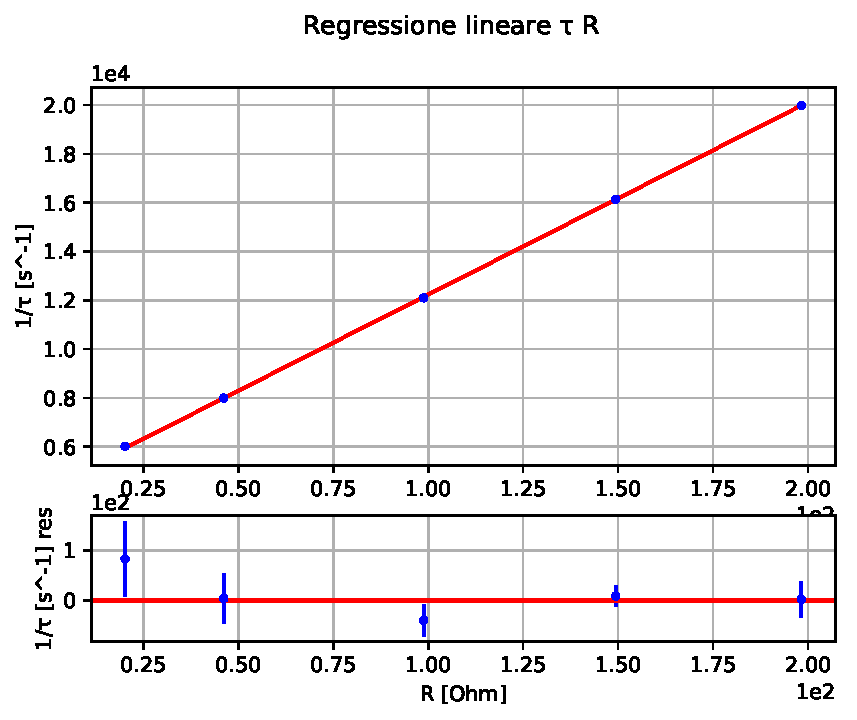
\includegraphics[width=0.5\textwidth]{fig_tau2.pdf}
	\caption{Curva di scarica esponenziale dell'induttore}
	\label{fig:fig_tau2}
\end{figure}

Essendo la relazione teorica di tipo lineare (\ref{eq:tauind}) , viene eseguita la regressione a due parametri e si estraggono le quantit\'a $\lambda$ e $\gamma$. Il $\chi$ quadrato corrispondente ($\chi^2_{r,3 \mathrm{dof}}=34$) mostra una possibile sottostima delle incertezze su $B$ e si procede quindi a moltiplicare le stesse per $\sqrt{\chi^2_r}$ in modo da imporre $\chi^2_r=1$.

\begin{center}
\begin{tabular}{c | c c }
	& Originale & Compatibilit\'a imposta \\
	\hline
 $\lambda \ [\si{\per\ohm\per\second}]$ & $4349\pm 7$  & $ (4.35\pm 0.04)\E{3} $\\
 $\gamma \ [\si{\per\second}]$ & $78.85\pm 0.05$ & $78.85\pm 0.31 $ \\
 $L = 1/\lambda \ [\si{\henry}]$ & $ (12.683 \pm 0.008)\E{3} $ & $ (12.68\pm 0.05)\E{3} $ \\
 $R_l = \gamma/\lambda - 50 \ [\si{\ohm}]$ & $5.16\pm 0.13$ & $5.2\pm 0.8$ \\
\end{tabular}
\end{center}

Il valore di $R_l$ misurato alla prima esperienza era di $0.51 \ \si{\ohm}$ e sembrerebbe quindi che ci sia un qualche tipo di discordanza con il risultato appena ottenuto. Una possibile spiegazione \'e che la misura tramite DMM della resistenza della bobina avviene in modo statico mentre in questo caso viene calcolata attraverso un'analisi delle caratteristiche dinamiche della stessa durante la scarica e quindi potrebbero nascere effetti che non sono stati presi in considerazione. Un ulteriore valore di $R_l$ verr\'a in seguito ottenuto osservando le caratteristiche del picco di risonanza del circuito RLC.

\FloatBarrier
\newpage
\subsection{Filtri RLC}

Si consideri ora il circuito passa banda RLC in figura \ref{fig:RLC}.

\begin{figure}[h!]
\begin{center}
    \begin{circuitikz} []
    \draw
        (4,0) node[ground] {} to [L, l=$L$] (4,2)
        (4,2) to [R, l=$R_l$] (4,4)
        (6,0) node[ground] {} to [C, l=$C_{tot}$] (6,4)
        (8,0) node[ground] {} to [R, l=$R_{osc}$] (8,4)
        (2,4) to [R, l=$R$] (4,4) to (9,4) node[right] {$V_{out}$}
        (2,4) node[left] {$V_{in}$}
        (2,4) to [open, *-*] (9,4);
        %(9,4) to [open, *-] (0,0);
    \end{circuitikz}
\end{center}
\caption{Circuito RLC}
\label{fig:RLC}
\end{figure}

\begin{gather*}
	C_{tot} = C + C_l + C_{osc}
\end{gather*}

Il valore della capacit\'a $C_l$ \'e stato ottenuto osservando la frequenza di risonanza LC alla quale il filtro produce un massimo di ampiezza in uscita nel caso in cui $C=0 \si{\farad}$ e risulta:

\begin{gather}
	\omega_0 = \frac{1}{\sqrt{L (C_l + C_{osc})}} = 7.19\E{5}\ \si{\radian \per \second}\\
	C_l = \frac{1}{\omega_0^2 L} - C_{osc} = 2.27\E{-11} \si{\farad}
\end{gather}

La capacit\'a $C_l$ viene presa senza incertezza in quanto sempre sommata alla capacit\'a $C$ il cui errore \'e molto maggiore.

Gli altri valori dei componenti che compaiono nel circuito sono: $R=466\ \&\ 9924.5\ \si{\ohm}$ , $C=32.89\E{-9} \si{\farad}$ , $C_{osc}=130\E{-12} \ \si{\farad}$ , $L=12.68\E{-3} \si{\henry}$ , $R_l=5.2 \ \si{\ohm}$.

Vengono ora mostrati i grafici di Bode dei due filtri a confronto con il modello teorico.

\begin{figure}[H]
    \centering
    \begin{minipage}{0.5\textwidth}
        \centering
        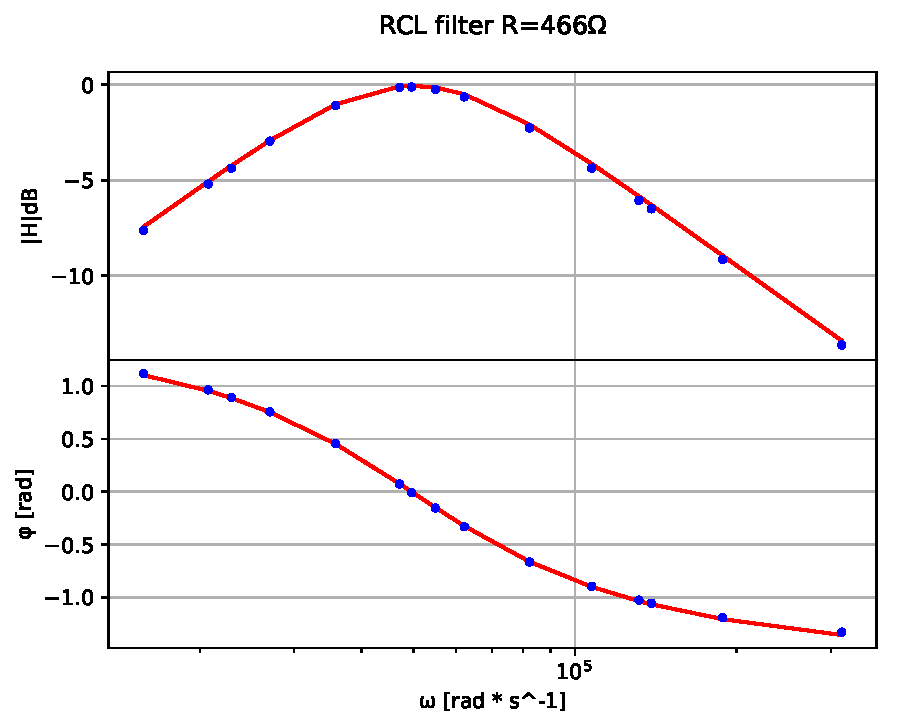
\includegraphics[width=\textwidth]{bodefilter1.pdf} 
        %\caption{first figure}
    \end{minipage}\hfill
    \begin{minipage}{0.5\textwidth}
        \centering
        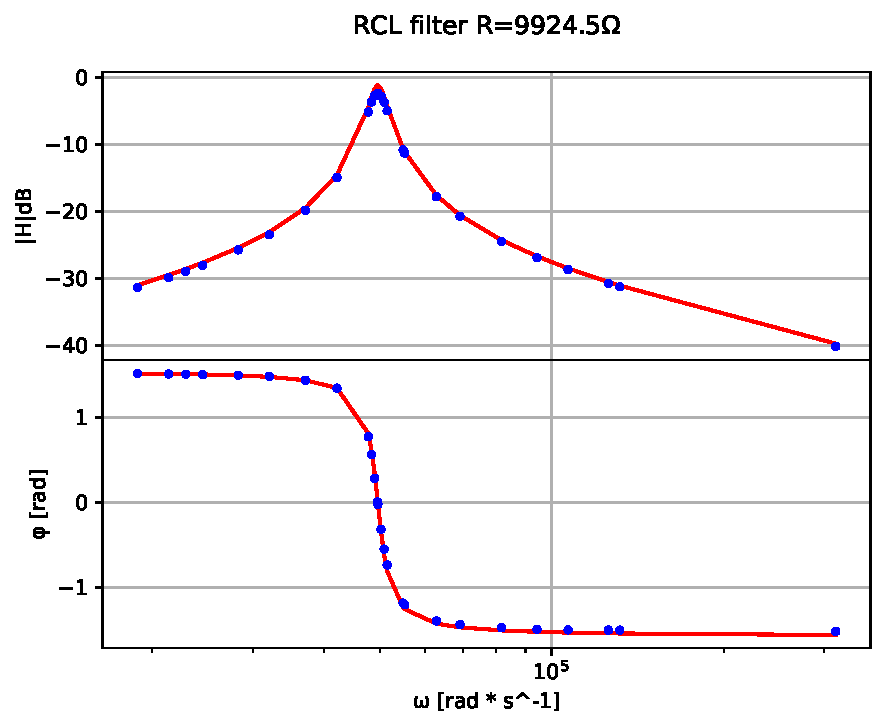
\includegraphics[width=\textwidth]{bodefilter2.pdf} 
        %\caption{second figure}
    \end{minipage}
    \\
    \centering
    \begin{minipage}{0.5\textwidth}
        \centering
        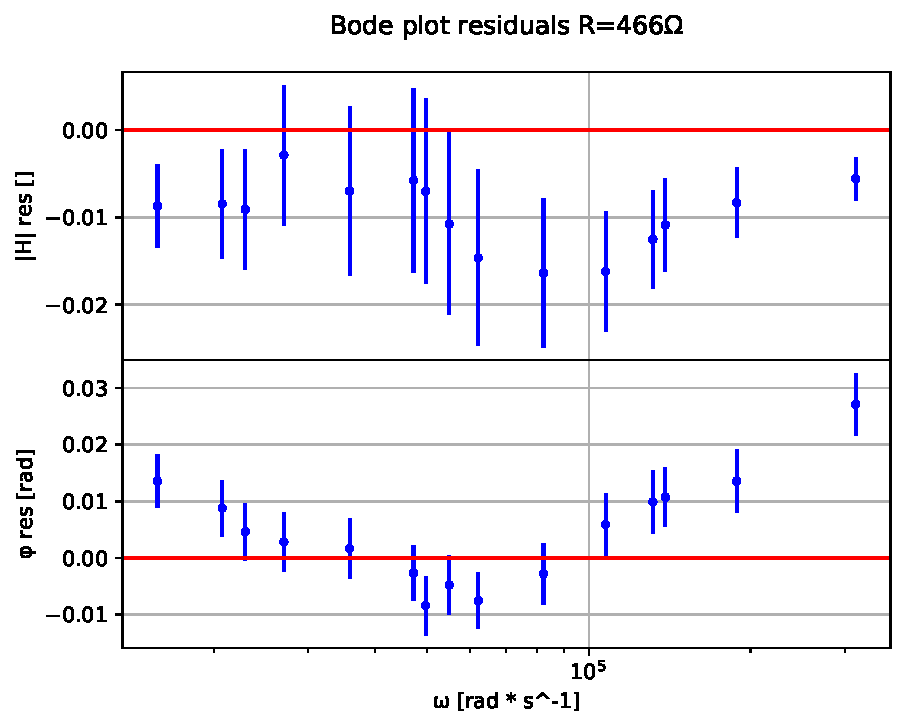
\includegraphics[width=\textwidth]{bodefilter1_res.pdf} 
        %\caption{first figure}
    \end{minipage}\hfill
    \begin{minipage}{0.5\textwidth}
        \centering
        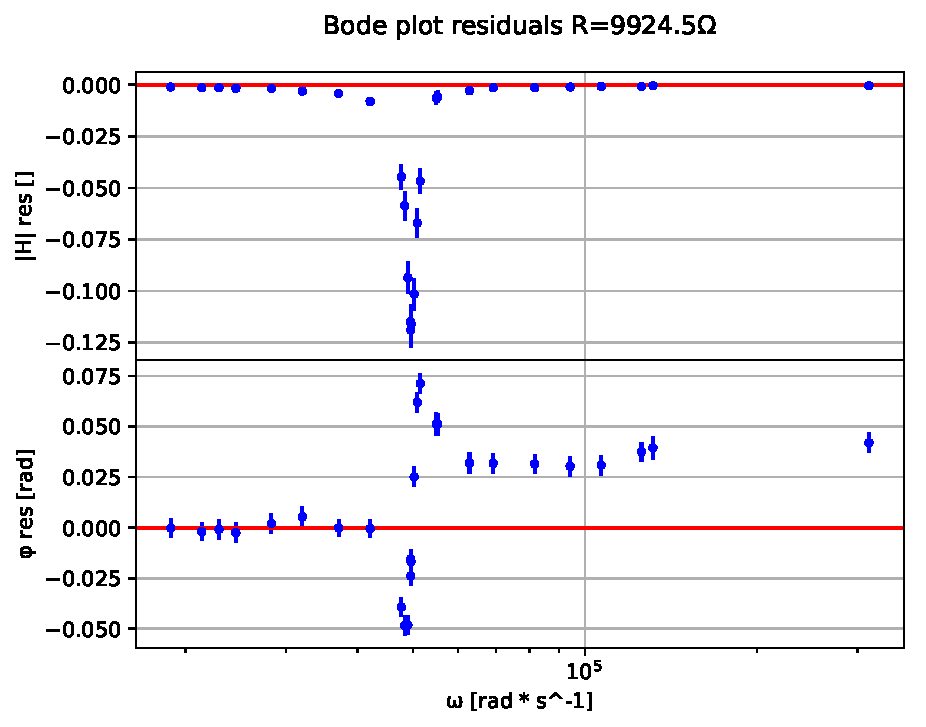
\includegraphics[width=\textwidth]{bodefilter2_res.pdf} 
        %\caption{second figure}
    \end{minipage}
    \caption{Grafici di Bode per i due filtri, in blu i punti sperimentali ed in rosso il modello teorico}
    \label{fig:RCLfilter}
\end{figure}

Come si pu\'o notare nel primo caso i residui si distribuiscono in modo sufficientemente uniforme e a meno di una minima sottostima delle incertezze quindi risponde come un passa alto a bassa frequenza e passa basso ad alta frequenza. Utilizzando invece la resistenza di valore maggiore i residui mostrano una pi\'u marcata deviazione dal modello, specialmente attorno al picco, e questo pu\'o essere spiegato da eventuali dissipazioni aggiuntive presenti, attriti magnetici nell'induttanza oppure da un sbagliato valore di $R_l$ proveniente dall'analisi svolta nel precedente capitolo.

Dalla teoria i parametri dei circuiti sono:

\begin{gather}
	\nonumber
	\omega_0 = \frac{1}{\sqrt{L(C+c_{osc}+C_l)}} = 49543\ \si{\radian\per\second} \\
	\nonumber
	Q = R \sqrt{\frac{C+C_{osc}+C_l}{L}} = 
	\begin{cases}  
	0.742 \ \mathrm{con} \  R=466\ \si{\ohm} \\
	15.8 \  \mathrm{con}\  R=9924.5\ \si{\ohm}
	\end{cases}
\end{gather}

Siamo ora interessati al comportamento specifico del secondo caso, il pi\'u selettivo, verr\'a quindi svolta una regressione ad una parabola, con parametri $A$, $B$ e $C$, del picco di risonanza nel grafico di Bode.

\begin{gather}
	\nonumber
	X=\log_{10}{\omega} \qquad
	Y=20 \log_{10}{|H|} \qquad
	\sigma[Y]=\frac{20}{\log{10}} \frac{\sigma[|H|]}{|H|} \\
	Y=A X^2 + B X + C \\
	\log_{10}{(\omega_0)} = \frac{-B}{2A} = \Omega \qquad 
	\log_{10}{(|H|_{max})} = \frac{A \Omega^2 + B \Omega + C}{20} \\
\end{gather}

I cui risultati sono esposti in figura \ref{fig:figp}.

\begin{figure}[h]
\centering
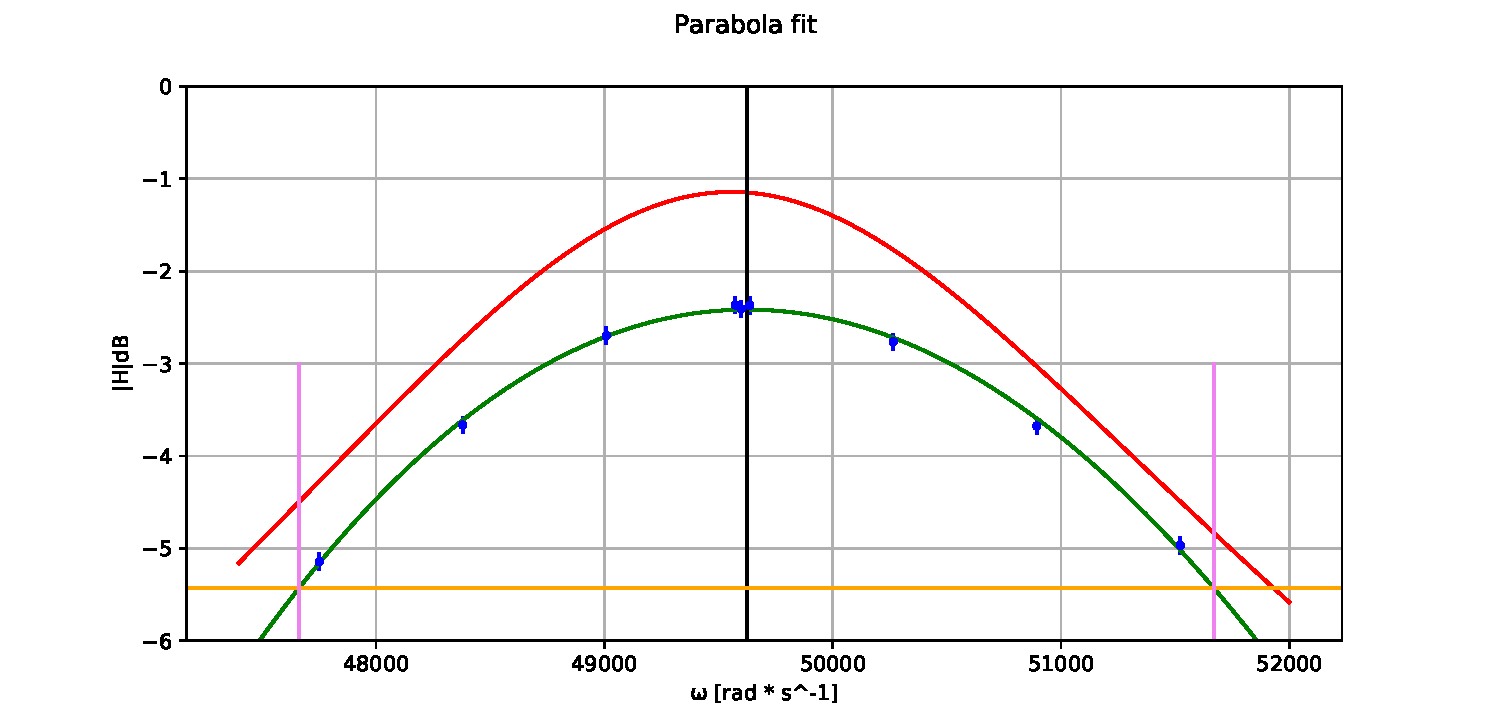
\includegraphics[width=\textwidth]{figp.pdf}
\caption{Regressione a parabola: in blu i punti sperimentali, in rosso la funzione di trasferimento teorica, in verde il risultato del fit a parabola, in nero $\omega_0$ di risonanza secondo il fit, in arancione ampiezza corrispondente a $|H|_{max}/\sqrt{2}$ ed in magenta le $\omega$ che determinano la larghezza del picco sempre secondo il fit}
\label{fig:figp}
\end{figure}

Infine per completare il confronto con la teoria si calcolano i parametri del circuito ricavati dal fit a parabola:

\begin{gather}
	\omega_0 = 49625 \ \si{\radian\per\second} \\
	Q = \frac{\omega_0}{\Delta \omega_{\textrm{3dB}}} = 12.4 \\ 
	|H|_{max} = 0.757 
\end{gather}

Inoltre ora pu\'o essere effettuata una nuova stima del parametro $R_l$ supposto, ragionevolmente, che $\omega_0$ non dipenda da $R_l$ o da $R_{osc}$.
Chiamata $Z$ l'impedenza dell'unione circuitale delle capacità parassite e non (qui chiamate $C$ per semplicit\'a), nonch\'e dell'induttanza e della sua $R_l$ interna, otteniamo:

\begin{gather}
	\nonumber
	\omega_0=1/\sqrt{LC} \\ 
	\nonumber
	Z = (R_l + j\omega L) \pars \frac{1}{j \omega C} = \frac{R_l+j\omega L}{1+j \omega R_l C - \omega^2 C L}\\
	\nonumber
	Z_0 = Z_{@ \omega_0} =  \frac{R_l + j \omega_0 L}{j\omega_0 R_l C} \\
	\label{eq:z0mod}
	|Z|^2_{0} = \frac{1}{\omega_0^2 C^2} + \frac{L^2}{R_l^2 C^2} \\
	\label{eq:h0mod}
	|H|_{0} =\frac{|Z|_0 \pars R_{osc}}{|Z|_0 \pars R_{osc} + R} = \frac{|Z|_0 R_{osc}}{|Z|_0 (R_{osc} + R) +R_{osc} R}
\end{gather}

Si suppone inoltre che $Z_0$ abbia parte immaginaria molto minore della parte reale (cosa che effettivamente succede) in modo da scrivere $H_0$, la funzione di trasferimento alla risonanza, come nell'equazione \ref{eq:h0mod}.

Si estrae quindi $R_l$ dall'equazione \ref{eq:z0mod} e $|Z|_0$ dalla \ref{eq:h0mod} per ottenere:

\begin{gather}
	|Z|_0 = \frac{|H|_0 R_{osc} R}{R_{osc} - |H|_0 (R_{osc}+R)} \\
	\bar{R_l} = \frac{L}{C} \sqrt{\frac{1}{|Z|^2_0 - \frac{1}{\omega_0^2 C^2}}} = 12.41 \ \si{\ohm} \ @ \ \omega_0
\end{gather}

Se questo nuovo valore $\bar{R_l}$ viene utilizzato per il grafico di Bode teorico della funzione di trasferimento a confronto con i dati sperimentali si ottiene la figura \ref{fig:bodeconfr}.

\begin{figure}[h]
\centering
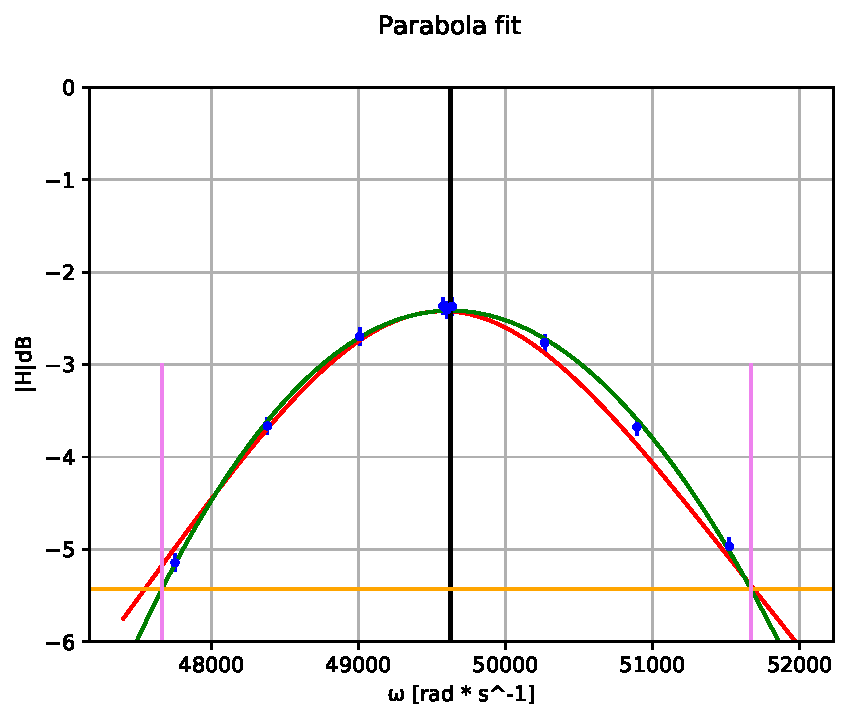
\includegraphics[width=0.6\textwidth]{bodeconf.pdf}
\caption{Nuova regressione a parabola}
\label{fig:bodeconfr}
\end{figure}
 
Come si pu\'o vedere la predizione teorica \'e molto pi\'u coerente con dati misurati questa volta. \\

Invece di aver ipotizzato una $R_l$ sottostimata, come \'e stato fatto, si sarebbe potuta interpretare la discrepanza come se l'induttanza presentasse un valore $L$ in possesso anche di una parte immaginaria che non compariva nella misura dovuta alla sua scarica.
In tal caso:

\begin{gather}
	\mathcal{L} = L + j\delta L \\
	\delta L = - \frac{\bar{R_l} - R_l}{\omega_0} = - 0.1453 \ \si{\milli\henry}
\end{gather}

\end{document}
